% Created by tikzDevice version 0.12 on 2019-03-22 17:55:14
% !TEX encoding = UTF-8 Unicode
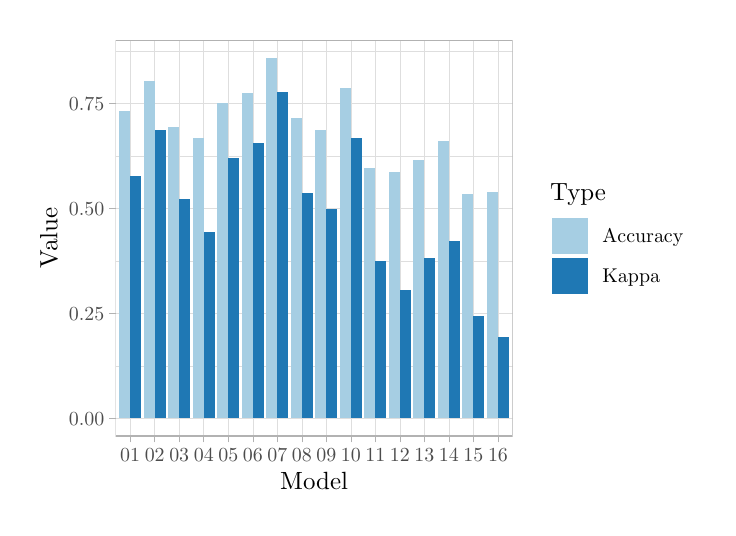
\begin{tikzpicture}[x=1pt,y=1pt]
\definecolor{fillColor}{RGB}{255,255,255}
\path[use as bounding box,fill=fillColor,fill opacity=0.00] (0,0) rectangle (245.72,173.45);
\begin{scope}
\path[clip] (  0.00,  0.00) rectangle (245.72,173.45);
\definecolor{drawColor}{RGB}{255,255,255}
\definecolor{fillColor}{RGB}{255,255,255}

\path[draw=drawColor,line width= 0.5pt,line join=round,line cap=round,fill=fillColor] ( -0.00,  0.00) rectangle (245.72,173.45);
\end{scope}
\begin{scope}
\path[clip] ( 31.74, 25.85) rectangle (175.25,168.95);
\definecolor{fillColor}{RGB}{255,255,255}

\path[fill=fillColor] ( 31.74, 25.85) rectangle (175.25,168.95);
\definecolor{drawColor}{gray}{0.87}

\path[draw=drawColor,line width= 0.1pt,line join=round] ( 31.74, 51.29) --
	(175.25, 51.29);

\path[draw=drawColor,line width= 0.1pt,line join=round] ( 31.74, 89.18) --
	(175.25, 89.18);

\path[draw=drawColor,line width= 0.1pt,line join=round] ( 31.74,127.07) --
	(175.25,127.07);

\path[draw=drawColor,line width= 0.1pt,line join=round] ( 31.74,164.96) --
	(175.25,164.96);

\path[draw=drawColor,line width= 0.2pt,line join=round] ( 31.74, 32.35) --
	(175.25, 32.35);

\path[draw=drawColor,line width= 0.2pt,line join=round] ( 31.74, 70.24) --
	(175.25, 70.24);

\path[draw=drawColor,line width= 0.2pt,line join=round] ( 31.74,108.13) --
	(175.25,108.13);

\path[draw=drawColor,line width= 0.2pt,line join=round] ( 31.74,146.01) --
	(175.25,146.01);

\path[draw=drawColor,line width= 0.2pt,line join=round] ( 37.05, 25.85) --
	( 37.05,168.95);

\path[draw=drawColor,line width= 0.2pt,line join=round] ( 45.91, 25.85) --
	( 45.91,168.95);

\path[draw=drawColor,line width= 0.2pt,line join=round] ( 54.77, 25.85) --
	( 54.77,168.95);

\path[draw=drawColor,line width= 0.2pt,line join=round] ( 63.63, 25.85) --
	( 63.63,168.95);

\path[draw=drawColor,line width= 0.2pt,line join=round] ( 72.49, 25.85) --
	( 72.49,168.95);

\path[draw=drawColor,line width= 0.2pt,line join=round] ( 81.35, 25.85) --
	( 81.35,168.95);

\path[draw=drawColor,line width= 0.2pt,line join=round] ( 90.21, 25.85) --
	( 90.21,168.95);

\path[draw=drawColor,line width= 0.2pt,line join=round] ( 99.07, 25.85) --
	( 99.07,168.95);

\path[draw=drawColor,line width= 0.2pt,line join=round] (107.92, 25.85) --
	(107.92,168.95);

\path[draw=drawColor,line width= 0.2pt,line join=round] (116.78, 25.85) --
	(116.78,168.95);

\path[draw=drawColor,line width= 0.2pt,line join=round] (125.64, 25.85) --
	(125.64,168.95);

\path[draw=drawColor,line width= 0.2pt,line join=round] (134.50, 25.85) --
	(134.50,168.95);

\path[draw=drawColor,line width= 0.2pt,line join=round] (143.36, 25.85) --
	(143.36,168.95);

\path[draw=drawColor,line width= 0.2pt,line join=round] (152.22, 25.85) --
	(152.22,168.95);

\path[draw=drawColor,line width= 0.2pt,line join=round] (161.08, 25.85) --
	(161.08,168.95);

\path[draw=drawColor,line width= 0.2pt,line join=round] (169.94, 25.85) --
	(169.94,168.95);
\definecolor{fillColor}{RGB}{31,120,180}

\path[fill=fillColor] ( 37.05, 32.35) rectangle ( 41.04,119.96);
\definecolor{fillColor}{RGB}{166,206,227}

\path[fill=fillColor] ( 33.07, 32.35) rectangle ( 37.05,143.35);
\definecolor{fillColor}{RGB}{31,120,180}

\path[fill=fillColor] ( 45.91, 32.35) rectangle ( 49.90,136.40);
\definecolor{fillColor}{RGB}{166,206,227}

\path[fill=fillColor] ( 41.93, 32.35) rectangle ( 45.91,154.13);
\definecolor{fillColor}{RGB}{31,120,180}

\path[fill=fillColor] ( 54.77, 32.35) rectangle ( 58.76,111.42);
\definecolor{fillColor}{RGB}{166,206,227}

\path[fill=fillColor] ( 50.79, 32.35) rectangle ( 54.77,137.59);
\definecolor{fillColor}{RGB}{31,120,180}

\path[fill=fillColor] ( 63.63, 32.35) rectangle ( 67.62, 99.75);
\definecolor{fillColor}{RGB}{166,206,227}

\path[fill=fillColor] ( 59.64, 32.35) rectangle ( 63.63,133.76);
\definecolor{fillColor}{RGB}{31,120,180}

\path[fill=fillColor] ( 72.49, 32.35) rectangle ( 76.48,126.43);
\definecolor{fillColor}{RGB}{166,206,227}

\path[fill=fillColor] ( 68.50, 32.35) rectangle ( 72.49,146.36);
\definecolor{fillColor}{RGB}{31,120,180}

\path[fill=fillColor] ( 81.35, 32.35) rectangle ( 85.33,131.68);
\definecolor{fillColor}{RGB}{166,206,227}

\path[fill=fillColor] ( 77.36, 32.35) rectangle ( 81.35,149.99);
\definecolor{fillColor}{RGB}{31,120,180}

\path[fill=fillColor] ( 90.21, 32.35) rectangle ( 94.19,150.36);
\definecolor{fillColor}{RGB}{166,206,227}

\path[fill=fillColor] ( 86.22, 32.35) rectangle ( 90.21,162.44);
\definecolor{fillColor}{RGB}{31,120,180}

\path[fill=fillColor] ( 99.07, 32.35) rectangle (103.05,113.74);
\definecolor{fillColor}{RGB}{166,206,227}

\path[fill=fillColor] ( 95.08, 32.35) rectangle ( 99.07,140.92);
\definecolor{fillColor}{RGB}{31,120,180}

\path[fill=fillColor] (107.92, 32.35) rectangle (111.91,107.89);
\definecolor{fillColor}{RGB}{166,206,227}

\path[fill=fillColor] (103.94, 32.35) rectangle (107.92,136.54);
\definecolor{fillColor}{RGB}{31,120,180}

\path[fill=fillColor] (116.78, 32.35) rectangle (120.77,133.48);
\definecolor{fillColor}{RGB}{166,206,227}

\path[fill=fillColor] (112.80, 32.35) rectangle (116.78,151.75);
\definecolor{fillColor}{RGB}{31,120,180}

\path[fill=fillColor] (125.64, 32.35) rectangle (129.63, 89.07);
\definecolor{fillColor}{RGB}{166,206,227}

\path[fill=fillColor] (121.66, 32.35) rectangle (125.64,122.79);
\definecolor{fillColor}{RGB}{31,120,180}

\path[fill=fillColor] (134.50, 32.35) rectangle (138.49, 78.56);
\definecolor{fillColor}{RGB}{166,206,227}

\path[fill=fillColor] (130.51, 32.35) rectangle (134.50,121.19);
\definecolor{fillColor}{RGB}{31,120,180}

\path[fill=fillColor] (143.36, 32.35) rectangle (147.35, 90.36);
\definecolor{fillColor}{RGB}{166,206,227}

\path[fill=fillColor] (139.37, 32.35) rectangle (143.36,125.79);
\definecolor{fillColor}{RGB}{31,120,180}

\path[fill=fillColor] (152.22, 32.35) rectangle (156.20, 96.36);
\definecolor{fillColor}{RGB}{166,206,227}

\path[fill=fillColor] (148.23, 32.35) rectangle (152.22,132.40);
\definecolor{fillColor}{RGB}{31,120,180}

\path[fill=fillColor] (161.08, 32.35) rectangle (165.06, 69.26);
\definecolor{fillColor}{RGB}{166,206,227}

\path[fill=fillColor] (157.09, 32.35) rectangle (161.08,113.48);
\definecolor{fillColor}{RGB}{31,120,180}

\path[fill=fillColor] (169.94, 32.35) rectangle (173.92, 61.76);
\definecolor{fillColor}{RGB}{166,206,227}

\path[fill=fillColor] (165.95, 32.35) rectangle (169.94,114.24);
\definecolor{drawColor}{gray}{0.70}

\path[draw=drawColor,line width= 0.5pt,line join=round,line cap=round] ( 31.74, 25.85) rectangle (175.25,168.95);
\end{scope}
\begin{scope}
\path[clip] (  0.00,  0.00) rectangle (245.72,173.45);
\definecolor{drawColor}{gray}{0.30}

\node[text=drawColor,anchor=base east,inner sep=0pt, outer sep=0pt, scale=  0.72] at ( 27.69, 29.87) {0.00};

\node[text=drawColor,anchor=base east,inner sep=0pt, outer sep=0pt, scale=  0.72] at ( 27.69, 67.76) {0.25};

\node[text=drawColor,anchor=base east,inner sep=0pt, outer sep=0pt, scale=  0.72] at ( 27.69,105.65) {0.50};

\node[text=drawColor,anchor=base east,inner sep=0pt, outer sep=0pt, scale=  0.72] at ( 27.69,143.53) {0.75};
\end{scope}
\begin{scope}
\path[clip] (  0.00,  0.00) rectangle (245.72,173.45);
\definecolor{drawColor}{gray}{0.70}

\path[draw=drawColor,line width= 0.2pt,line join=round] ( 29.49, 32.35) --
	( 31.74, 32.35);

\path[draw=drawColor,line width= 0.2pt,line join=round] ( 29.49, 70.24) --
	( 31.74, 70.24);

\path[draw=drawColor,line width= 0.2pt,line join=round] ( 29.49,108.13) --
	( 31.74,108.13);

\path[draw=drawColor,line width= 0.2pt,line join=round] ( 29.49,146.01) --
	( 31.74,146.01);
\end{scope}
\begin{scope}
\path[clip] (  0.00,  0.00) rectangle (245.72,173.45);
\definecolor{drawColor}{gray}{0.70}

\path[draw=drawColor,line width= 0.2pt,line join=round] ( 37.05, 23.60) --
	( 37.05, 25.85);

\path[draw=drawColor,line width= 0.2pt,line join=round] ( 45.91, 23.60) --
	( 45.91, 25.85);

\path[draw=drawColor,line width= 0.2pt,line join=round] ( 54.77, 23.60) --
	( 54.77, 25.85);

\path[draw=drawColor,line width= 0.2pt,line join=round] ( 63.63, 23.60) --
	( 63.63, 25.85);

\path[draw=drawColor,line width= 0.2pt,line join=round] ( 72.49, 23.60) --
	( 72.49, 25.85);

\path[draw=drawColor,line width= 0.2pt,line join=round] ( 81.35, 23.60) --
	( 81.35, 25.85);

\path[draw=drawColor,line width= 0.2pt,line join=round] ( 90.21, 23.60) --
	( 90.21, 25.85);

\path[draw=drawColor,line width= 0.2pt,line join=round] ( 99.07, 23.60) --
	( 99.07, 25.85);

\path[draw=drawColor,line width= 0.2pt,line join=round] (107.92, 23.60) --
	(107.92, 25.85);

\path[draw=drawColor,line width= 0.2pt,line join=round] (116.78, 23.60) --
	(116.78, 25.85);

\path[draw=drawColor,line width= 0.2pt,line join=round] (125.64, 23.60) --
	(125.64, 25.85);

\path[draw=drawColor,line width= 0.2pt,line join=round] (134.50, 23.60) --
	(134.50, 25.85);

\path[draw=drawColor,line width= 0.2pt,line join=round] (143.36, 23.60) --
	(143.36, 25.85);

\path[draw=drawColor,line width= 0.2pt,line join=round] (152.22, 23.60) --
	(152.22, 25.85);

\path[draw=drawColor,line width= 0.2pt,line join=round] (161.08, 23.60) --
	(161.08, 25.85);

\path[draw=drawColor,line width= 0.2pt,line join=round] (169.94, 23.60) --
	(169.94, 25.85);
\end{scope}
\begin{scope}
\path[clip] (  0.00,  0.00) rectangle (245.72,173.45);
\definecolor{drawColor}{gray}{0.30}

\node[text=drawColor,anchor=base,inner sep=0pt, outer sep=0pt, scale=  0.72] at ( 37.05, 16.84) {01};

\node[text=drawColor,anchor=base,inner sep=0pt, outer sep=0pt, scale=  0.72] at ( 45.91, 16.84) {02};

\node[text=drawColor,anchor=base,inner sep=0pt, outer sep=0pt, scale=  0.72] at ( 54.77, 16.84) {03};

\node[text=drawColor,anchor=base,inner sep=0pt, outer sep=0pt, scale=  0.72] at ( 63.63, 16.84) {04};

\node[text=drawColor,anchor=base,inner sep=0pt, outer sep=0pt, scale=  0.72] at ( 72.49, 16.84) {05};

\node[text=drawColor,anchor=base,inner sep=0pt, outer sep=0pt, scale=  0.72] at ( 81.35, 16.84) {06};

\node[text=drawColor,anchor=base,inner sep=0pt, outer sep=0pt, scale=  0.72] at ( 90.21, 16.84) {07};

\node[text=drawColor,anchor=base,inner sep=0pt, outer sep=0pt, scale=  0.72] at ( 99.07, 16.84) {08};

\node[text=drawColor,anchor=base,inner sep=0pt, outer sep=0pt, scale=  0.72] at (107.92, 16.84) {09};

\node[text=drawColor,anchor=base,inner sep=0pt, outer sep=0pt, scale=  0.72] at (116.78, 16.84) {10};

\node[text=drawColor,anchor=base,inner sep=0pt, outer sep=0pt, scale=  0.72] at (125.64, 16.84) {11};

\node[text=drawColor,anchor=base,inner sep=0pt, outer sep=0pt, scale=  0.72] at (134.50, 16.84) {12};

\node[text=drawColor,anchor=base,inner sep=0pt, outer sep=0pt, scale=  0.72] at (143.36, 16.84) {13};

\node[text=drawColor,anchor=base,inner sep=0pt, outer sep=0pt, scale=  0.72] at (152.22, 16.84) {14};

\node[text=drawColor,anchor=base,inner sep=0pt, outer sep=0pt, scale=  0.72] at (161.08, 16.84) {15};

\node[text=drawColor,anchor=base,inner sep=0pt, outer sep=0pt, scale=  0.72] at (169.94, 16.84) {16};
\end{scope}
\begin{scope}
\path[clip] (  0.00,  0.00) rectangle (245.72,173.45);
\definecolor{drawColor}{RGB}{0,0,0}

\node[text=drawColor,anchor=base,inner sep=0pt, outer sep=0pt, scale=  0.90] at (103.50,  6.44) {Model};
\end{scope}
\begin{scope}
\path[clip] (  0.00,  0.00) rectangle (245.72,173.45);
\definecolor{drawColor}{RGB}{0,0,0}

\node[text=drawColor,rotate= 90.00,anchor=base,inner sep=0pt, outer sep=0pt, scale=  0.90] at ( 10.70, 97.40) {Value};
\end{scope}
\begin{scope}
\path[clip] (  0.00,  0.00) rectangle (245.72,173.45);
\definecolor{fillColor}{RGB}{255,255,255}

\path[fill=fillColor] (184.25, 72.12) rectangle (241.22,122.67);
\end{scope}
\begin{scope}
\path[clip] (  0.00,  0.00) rectangle (245.72,173.45);
\definecolor{drawColor}{RGB}{0,0,0}

\node[text=drawColor,anchor=base west,inner sep=0pt, outer sep=0pt, scale=  0.90] at (188.75,111.00) {Type};
\end{scope}
\begin{scope}
\path[clip] (  0.00,  0.00) rectangle (245.72,173.45);
\definecolor{fillColor}{RGB}{255,255,255}

\path[fill=fillColor] (188.75, 91.08) rectangle (203.21,105.53);
\end{scope}
\begin{scope}
\path[clip] (  0.00,  0.00) rectangle (245.72,173.45);
\definecolor{fillColor}{RGB}{166,206,227}

\path[fill=fillColor] (189.46, 91.79) rectangle (202.49,104.82);
\end{scope}
\begin{scope}
\path[clip] (  0.00,  0.00) rectangle (245.72,173.45);
\definecolor{fillColor}{RGB}{255,255,255}

\path[fill=fillColor] (188.75, 76.62) rectangle (203.21, 91.08);
\end{scope}
\begin{scope}
\path[clip] (  0.00,  0.00) rectangle (245.72,173.45);
\definecolor{fillColor}{RGB}{31,120,180}

\path[fill=fillColor] (189.46, 77.33) rectangle (202.49, 90.36);
\end{scope}
\begin{scope}
\path[clip] (  0.00,  0.00) rectangle (245.72,173.45);
\definecolor{drawColor}{RGB}{0,0,0}

\node[text=drawColor,anchor=base west,inner sep=0pt, outer sep=0pt, scale=  0.72] at (207.71, 95.82) {Accuracy};
\end{scope}
\begin{scope}
\path[clip] (  0.00,  0.00) rectangle (245.72,173.45);
\definecolor{drawColor}{RGB}{0,0,0}

\node[text=drawColor,anchor=base west,inner sep=0pt, outer sep=0pt, scale=  0.72] at (207.71, 81.37) {Kappa};
\end{scope}
\end{tikzpicture}
